\chapter{Metodología}
\label{chap:metodologia}



 %De acuerdo a \cite{Barrett2009}, el modelo WCM...\\
 
En esta tesis se dise\~nar\'a el procedimiento y el prototipo de software para el an\'alisis de una situaci\'on de encuentro entre una misi\'on primaria y un desecho espacial.\\
Partimos de la recepci\'on de un mensaje de alerta, proveniente de un organismo externo (JSpOC), en formato CDM. La primera instancia consiste en extraer la informaci\'on que permita identificar la nave propia, el desecho espacial involucrado y el instante en que se estima el encuentro \ac{TCA}. Ya con esta informaci\'on se puede hacer la solicitud de los TLE a space-track para empezar el an\'alisis de la situaci\'on y se solicitan a Din\'amica Orbital las efem\'erides precisas necesarias.\\
El siguiente paso implica desarrollar un m\'etodo que ajuste los TLE, mejore la estimaci\'on de la posici\'on del desecho y calcule los errores asociados.\\
Finalmente se calcular\'a el par\'ametro de \ac{PoC}, como indicador cuantitativo del nivel del riesgo.\\

Para el desarrollo del prototipo de software ARxCODE, se propone una metodolog\'ia evolutiva incremental, basada en la construcci\'on de distintos m\'odulos que resuelvan las etapas planteadas. Los mismos ir\'an valid\'andose y perfeccion\'andose durante el proceso, de manera independiente pero enmarcados en una arquitectura y dise\~no que se resolver\'a en las primeras etapas.\\
Se listan a continuaci\'on los tres principales m\'odulos a desarrollar:\\ 
%Se plasma una estructura/arquitectura de alto nivel consolidada, cuyas interfaces con: SW de Dinámica Orbital de CUSS y otros entes, queda estipulada y se atomizan estructuras internas, capaces de ser actualizadas y cuyas interacciones sean versátiles.\\

\begin{itemize}
\item M\'odulo de ajuste y correcci\'on de la posici\'on del desecho espacial.\\
\item M\'odulo de c\'alculo de la PoC.\\
\item M\'odulo de administraci\'on del CDM.\\
\item M\'odulo de administraci\'on de los datos provistos por el departamento de Din\'amica Orbital.\\
\end{itemize}

% \begin{figure}[!h]
% \centering
% \includegraphics[width=\textwidth]{../imagenes/arxcodencuentros11}
% \caption{Arquitectura de alto nivel del ARxCODE}
% \end{figure}


\subsection*{M\'odulo de ajuste y correcci\'on de la posici\'on del desecho.}
Si bien la base de datos de NORAD, pone a disposici\'on p\'ublica la informaci\'on orbital de los objetos en formato TLE, se desconocen los errores asociados a esa determinaci\'on orbital, al igual que los que introduce la propagaci\'on de los mismos con el modelo de propagaci\'on compatible SGP4.\\
En este m\'odulo esta tesis ofrece una nueva variante para la estimaci\'on de errores en la propagaci\'on de \'orbitas de desechos a partir de TLE.\\
Se utiliza el conjunto de los \'ultimos TLE publicados y se calculan las diferencias en la posici\'on, utilizando el \'ultimo TLE m\'as cercano a la fecha del TCA, como se propone en el trabajo de Osweiler \cite{osweiler}. El m\'etodo utiliza un conjunto de TLE de un dado objeto, por el periodo de 2 semanas. A partir de la propagaci\'on con SGP4 calcula las diferencias en las posiciones y velocidades contra un vector de estado estimado, a fin de caracterizar el comportamiento de la varianza y la matriz de covarianza para el TLE m\'as reciente.\\
A partir de esos resultados se realiza un ajuste por m\'inimos cuadrados y se propone una funci\'on de corrección.\\

\subsection*{M\'odulo de cálculo de la PoC.}
%Pasos comunes a todos los m\'etodos.\\
La PoC es el par\'ametro estad\'istico final que nos permitir\'a evaluar cuantitativamente la situaci\'on.\\
Optamos por la PoC ya que muestra mayor confiabilidad que otros par\'ametros, como por ejemplo la miss distance (m\'inima distancia), dado que la miss distance no contempla errores de propagaci\'on y genera sobrestimaci\'on de encuentros.\\
Los c\'alculos probabil\'isticos para este tipo de problemas en tres dimensiones resultan de pesada carga computacional, por lo que conviene usar t\'ecnicas de reducci\'on del problema a dos dimensiones o a un plano de encuentro \cite{foster}. Para el c\'alculo de la PoC se utilizar\'a el m\'etodo de Akella \cite{akellaAlfriend} ya que es conceptualmente simple y aunque tiene un alto costo computacional, es realizable por las m\'aquinas actuales en tiempos menores a un segundo.\\
%El procedimiento general frente a un posible enuentro consiste en propagar las \'orbitas y recalcular la situaci\'on de acercamiento a medida que se aproxima la fecha de la posible colisi\'on. Todo esto  con una antelaci\'on prudencial que permita la planificaci\'on de la maniobra, si \'esta resultara inevitablemente necesaria.

\subsection*{M\'odulo de administraci\'on de los datos provistos por el departamento de Din\'anica Orbital.}
Consiste en la solicitud/extracci\'on de los datos orbitales con la mayor precisi\'on posible que puedan obtenerse, propagados al momento del encuentro.\\
S\'olo ser\'a un m\'odulo de gesti\'on de datos que interactuar\'a con la base de datos de Din\'amica Orbital.\\ 


\subsection*{M\'odulo de administraci\'on del CDM.}
Este m\'odulo ser\'a el encargado de la detecci\'on y el desglose de la informaci\'on del CDM que provee JSpOC.\\
El mismo ofrecer\'a al operador usuario una visualizaci\'on resumida de la situaci\'on con la informaci\'on m\'as importante, y operar\'a de interfaz con el resto del sistema ARxCODE, provey\'endole los datos iniciales necesarios a los siguientes m\'odulos. A saber:\\

\begin{itemize}
\item Identificador de la  misi\'on primaria.
\item Identificador del desecho espacial.
\item TCA.
\item PoC.
\end{itemize}  

Una vez finalizados y validados los m\'odulos, resta la integraci\'on y la verificaci\'on de las distintas interfaces.\\


%\subsection*{Ajuste de TLEs - Osweiler}
%Genera a su vez, una relaci\'on de autocorrelaci\'on, que permite hacer una estimaci\'on del nivel de confiabilidad de la predicci\'on orbital.\\
%{\bf{Teor\'ia de la Estimaci\'on:}}\\
%considera: \\
%\begin{itemize}
%\item Teorema Central del L\'imite.
%\item Teor\'ia de probabilidad multidimensional.
%\item Funciones de Distribuci\'on Gauseana.
%\item El operador Esperanza.
%\item T\'ecnicas de linalizaci\'on para sistemas din\'amicos no lineales.
%\item M\'inimos Cuadradados y Principio de M\'axima Probabilidad.
%\end{itemize}

%{\bf{Ma. Covarianza:}}\\

%COV[v]=E
%\[
%\begin{bmatrix}
%(x-E[x])(x-E[x]) & (x-E[x])(y-E[y]) & (x-E[x])(z-E[z])\\
%(y-E[y])(x-E[x]) & (y-E[y])(y-E[y]) & (y-E[y])(z-E[z])\\
%(z-E[z])(x-E[x]) & (z-E[z])(y-E[y]) & (z-E[z])(z-E[z])
%\end{bmatrix}
%\]
%=
%\(
%\begin{pmatrix}
%Var[x] & Cov[x,y] & Cov[x,z]\\
%Cov[y,x] & Var[y] & Cov[y,z]\\
%Cov[z,x] & Cov[z,y] & Var[z]
%\end{pmatrix}
%\)


%El {\it{Teorema Central del L\'imite}} justifica la consideraci\'on de que el error estad\'istico de las mediciones sea Gauseano.

%\subsubsection*{Ma. de Covarianza}
%\begin{itemize}
%\item Se calculan los errores $e$ para las 10 fechas, correspondientes a los TLEs, para cada una de las variables $ex, ey, ez$.\\
%\item Se calcula la media de los errores $mx, my, mz$.\\
%\item ...
%\end{itemize}


 


\section{M\'etodo de Osweiler}
Es un m\'etodo que propone una manera de estimar los errores que se comenten en la utilizaci\'on de TLEs para la determinaci\'on de la posici\'on y la velocidad.
 El mismo consiste en utilizar un set de TLEs de un intervalo de dos semanas, y considerar el TLE m\'as pr\'oximo al tiempo de m\'aximo acercamiento (TLE  {\it{Primario}}) como el valor {\it{real}} o {\it{verdadero}}.\\
 A partir de esa premisa, propaga los TLEs anteriores hasta la \'epoca del TLE Primario y con las diferencias que resultan de la comparaci\'on, realiza los c\'alculos estad\'idticos de los valores medios y las varianzas, para construir la matriz Varianza Covarianza correpondiente al TLE Primario.\\
 Para hacer los estudios de validaci\'on de nuestra implementaci\'on del m\'etodo, de los 6 sat\'elites estudiados por Osweiler, dentro de 8 ventanas temporales distintas, nosotros hemos aplicado el m\'etodo a dos de ellos con caracter\'isticas similares a las misiones de CONAE y en particular a la misi\'on SAC-D, que hemos incorporamos como escenario propio de valiaci\'on ya que contamos con datos orbitales reales de mayor precisi\'on que los TLEs.

\section{Tratamiento sobre Datos de Misi\'on}
En esta etapa repetimos el m\'etodo que propone Osweiler considerando los datos de misi\'on generados por el CODS
como posici\'on verdadera.\\
La aplicaci\'on del m\'etodo implica:
\begin{itemize}
 \item Identificar el \'ultimo TLE del set: {\it{TLE primario.}}
 \item Extraer la \'epoca del TLE primario.
 \item Localizar el archivo CODS que contenga las efem\'erides que encierren la \'epoca del TLE primario.
 \item Interpolar las efem\'erides de CODS para generar una efem\'eride interpolada a la \'epoca del TLE primario.
 \item Propagar cada uno de los TLEs del set, hasta la \'epoca del TLE primario.
 \item Comparar los resultados de las propagaciones con los valores de la efem\'erides interpolada.
\end{itemize}

\begin{figure}[!h]
 \centering
 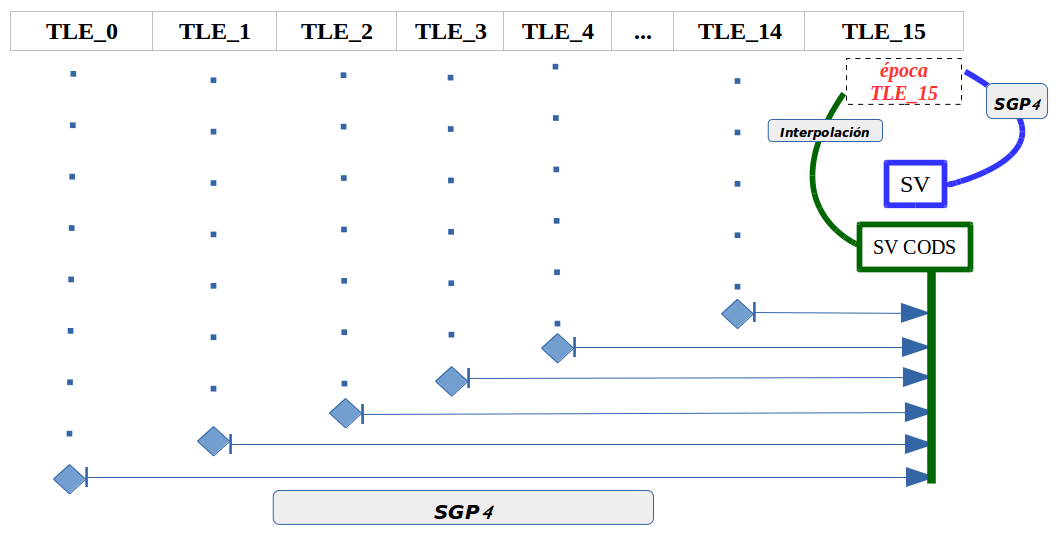
\includegraphics[width=0.7\textwidth]{imagenes/Osweiler_sobre_Cods.png}
 \caption{M\'etodo de Osweiler sobre datos CODS}
\end{figure}

\section{Preprocesamiento de los Datos de Misi\'on de CODS}
Para este trabajo CONAE nos facilit\'o el acceso a los datos orbitales de la misi\'on SAC-D.
Los datos se ecuentran montados en un servidor que contiene la informaci\'on organizada en archivos con formato ASCII, distribuidos en distintas carpetas seg\'un su clasificaci\'on.\\
Para la comparaci\'on que proponemos, solicitamos acceso a los archivos de efem\'erides orbitales ORBEPHEM, que ofrecen posiciones y velocidades tabuladas cada un minuto, en el Sistema de Referencia TOD (True of Date), en coordenadas cartesianas.

\subsection{ORBEPHEM}
Estos productos son generados luego de un post procesamiento que incluye una propagaci\'on ajustada por una determinaci\'on orbital. 
Cada archivo contiene un listado cronol\'ogicamente tabulado de posiciones y velocidades, dentro de un periodo de casi 3 d\'ias. ( doc\_interfaces)

La nomenclatura de los mismos respeta el siguiente formato:\\
\begin{verbatim}
 CODS_YYYYMMDD_HHMMSS_SACD_ORBEPHEM_TOD_XYZ_O.TXT
 
 Donde:
  CODS = Identifica el Servicio dentro del CUSS que presta la información.
  YYYYMMDD_HHMMSS = epoca de generación del dato.
  SACD = Identificación del Satélite.
  ORBEPHEM = Tipo de Dato, Efeméride Orbital (procesada a posteriori)
  TOD = Sistema de Referencia True of Date.
  XYZ = Tipo de efeméride, cartesiana.
  O = Operacional. 
\end{verbatim}


\subsection{Archivos Utilizados}
Si bien la nomenclatura de los archivos respeta una estructura, s\'olo se indica en el nombre, la fecha de generaci\'on de los datos y no puede desprenderse del mismo cu\'al es la \'epoca final e inicial de cada archivo, y no existe un registro del los gaps de datos ausentes. A su vez, las \'epocas contempladas en cada uno de ellos no está homogeneizada. Es decir, la fecha y hora inicial y final de cada registro es diferente para cada archivo.\\
Dada esta organizaci\'on, para el punto tres del procedimiento, referente a la localizaci\'on del archivo necesario para la comparaci\'on, la b\'usqueda se realiza de la siguiente manera:\\
Localizamos en primer lugar el archivo cuyo nombre coincide con la fecha de la \'epoca del TLE primario.
Como una misma fecha se encuentra en m\'as de un archivo, buscamos el archivo que contenga esa fecha y que adem\'as sea el m\'as actualizado de todos. Para ello, además del archivo cuyo nombre contiene la fecha del TLE primario, se enlistan los siguientes dos archivos y se ordenan en orden decreciente, de manera que el primer lugar de la lista lo ocupe el \'ultimo de los archivos seleccionados. Finalmente se comienza el proceso iterativo de abrir los archivos, evaluar el contenido y ver si se encuentran los dos registros que encierren la \'epoca del TLE.
Una vez que se encuentran las l\'ineas de efem\'erides que contienen la \'epoca de inter\'es se interpola, y se termina la iteraci\'on.

\noindent
Cantidad TOTAL de archivos $=  1454$\\
Cantidad media de resgistros por archivo $=  2688$\\
Archivo con el mayor n\'umero de registros $=  3042$\\
Archivo con el menor n\'umero de registros $=  142$\\

Im\'agenes comparativas entre los dos m\'etodos:\\

\begin{figure}[htbp]
 \centering
  \subfigure[Procesamiento de Datos de Mision]{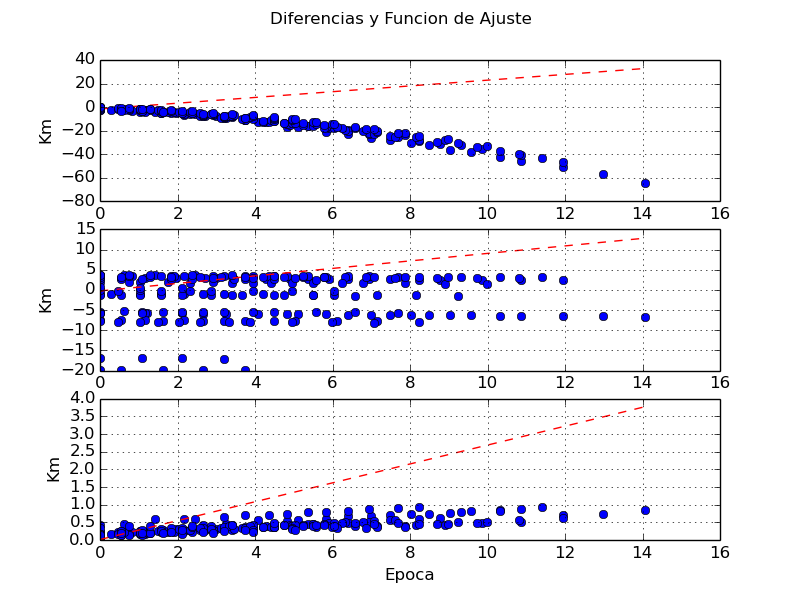
\includegraphics[width=0.46\linewidth]{imagenes/CODS_setCom_37673U_2}}
  \subfigure[Procesamiento de TLEs]{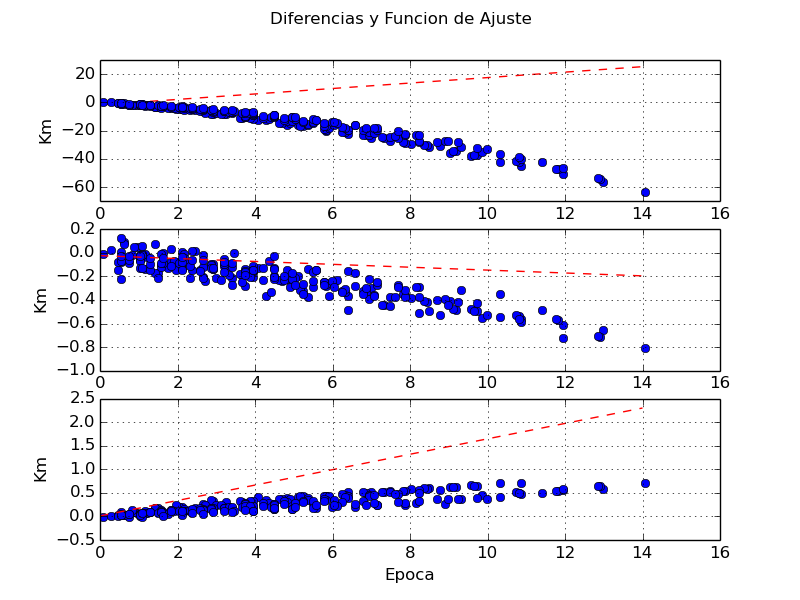
\includegraphics[width=0.46\linewidth]{imagenes/TLE_setCom_37673_2}}
 \caption{Resultado del m\'etodo de Pair-Wise Differencing considerando TLEs y Datos de Misi\'on.}
 \label{fig:test}
\end{figure}

\begin{verbatim}
------------------------------------------------------------------------
DIFERENCIAS: TLE-CODS
-------------------------------------------------------------------------
dv = -46.8489636874
dn = 2.35761559016
dc = 0.611728098324
\end{verbatim}

\begin{figure}[htbp]
 \centering
  \subfigure[Procesamiento de Datos de Mision]{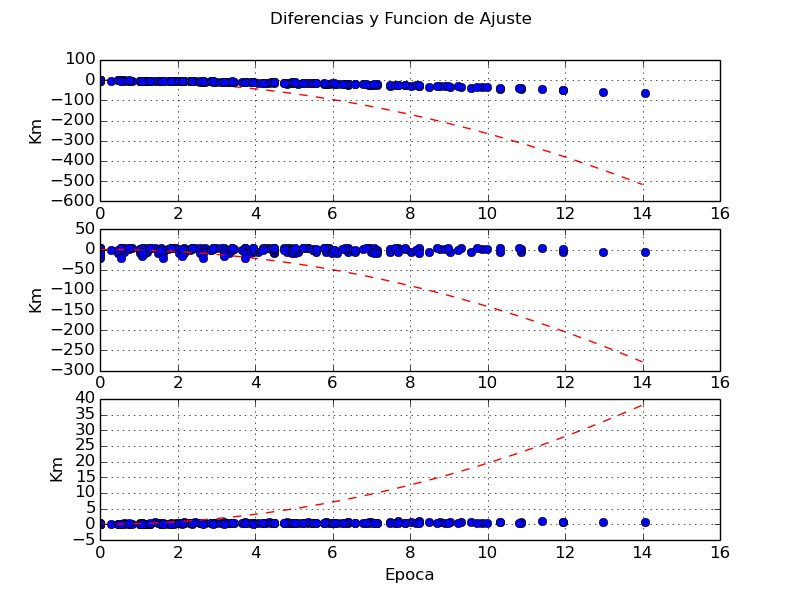
\includegraphics[width=0.46\linewidth]{imagenes/CODS_setCom_37673U_3}}
  \subfigure[Procesamiento de TLEs]{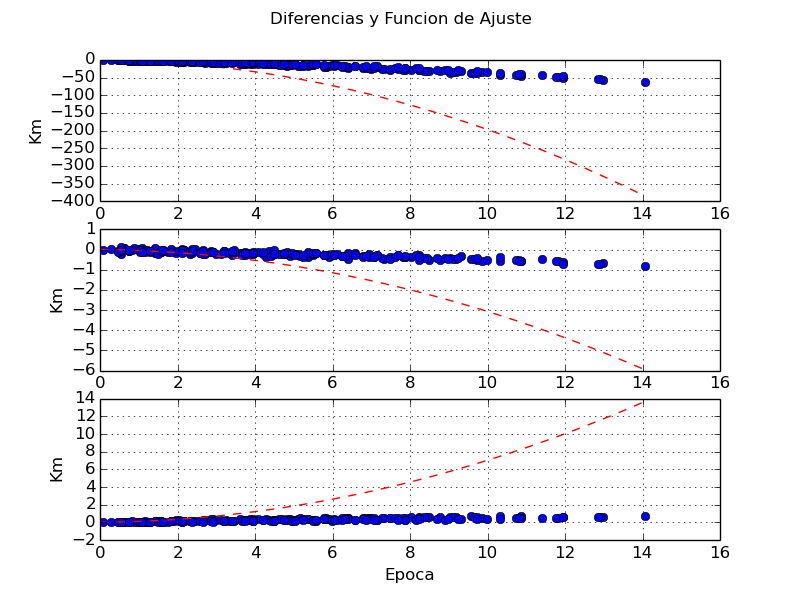
\includegraphics[width=0.46\linewidth]{imagenes/TLE_setCom_37673_3}}
 \caption{Resultado del m\'etodo de Pair-Wise Differencing considerando TLEs y Datos de Misi\'on.}
 \label{fig:test}
\end{figure}

\subsubsection{Ajuste Polyfit}

{\bf{numpy.polynomial.polynomial.polyfit}}

Returns:	

coef : ndarray, shape (deg + 1,) or (deg + 1, K)

    Polynomial coefficients ordered from low to high. If y was 2-D, the coefficients in column k of coef represent the polynomial fit to the data in y‘s k-th column.

residuals, rank, singular\_values, rcond : list

    These values are only returned if full = True

    resid – sum of squared residuals of the least squares fit rank – the numerical rank of the scaled Vandermonde matrix sv – singular values of the scaled Vandermonde matrix rcond – value of rcond.

    For more details, see linalg.lstsq.

\begin{verbatim}
Procesando datos TLE...
++++++++++++GRADO 2++++++++++++++++++
[array([-1.89669503, -0.73973919, -0.06103362])]
[[array([ 31434.82805686]), 3, array([ 1.68700379,  0.388,  0.056]), 5.1292e-14]]
++++++++++++GRADO 1++++++++++++++++++
[array([ 1.93247211, -1.78532883])]
[[array([ 31556.32886285]), 2, array([ 1.393,  0.24171176]), 5.1292e-14],]
\end{verbatim}

% \section{Graficos LAGEOS 8820}
% 
% \begin{figure}[H]
%  \centering
% \begin{subfigure}%{0.5\textwidth}
%   \centering
%   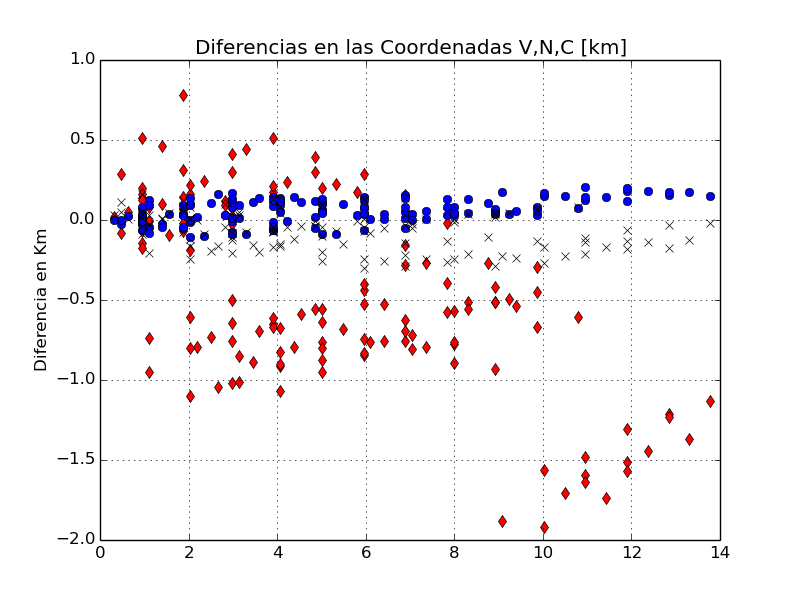
\includegraphics[width=0.7\linewidth]{imagenes/difTot8820.png}
%   \caption{A subfigure}
%   \label{fig:sub1}
% \end{subfigure}%
% \begin{subfigure}%{0.5\textwidth}
%   \centering
%   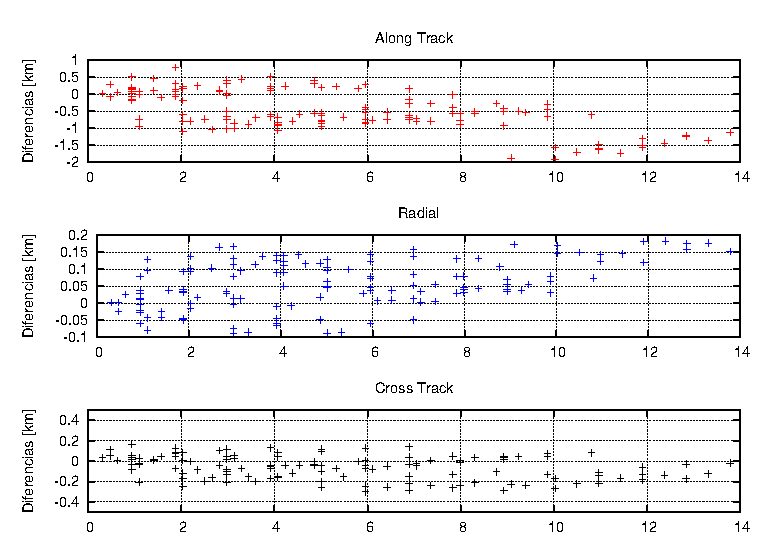
\includegraphics[width=0.7\linewidth]{imagenes/vncmultiplot}
%   \caption{A subfigure}
%   \label{fig:sub2}
% \end{subfigure}
% \caption{A figure with two subfigures}
% \label{fig:test}
% \end{figure}

\section{Transformaci\'on de Coordenadas}
[Montenbruck, Vallado Revisitin, Vallado Coorde Sys, tabla de Boado]

Para la comparaci\'on de las posiciones en coordenadas cartesianas, es necesario llevar ambos vectores a un mismo sistema de referencia.
La figura (ref) muestra un resumen de los distintos sistemas y las consideraciones de cada uno. 

\begin{figure}[!h]
  \centering
  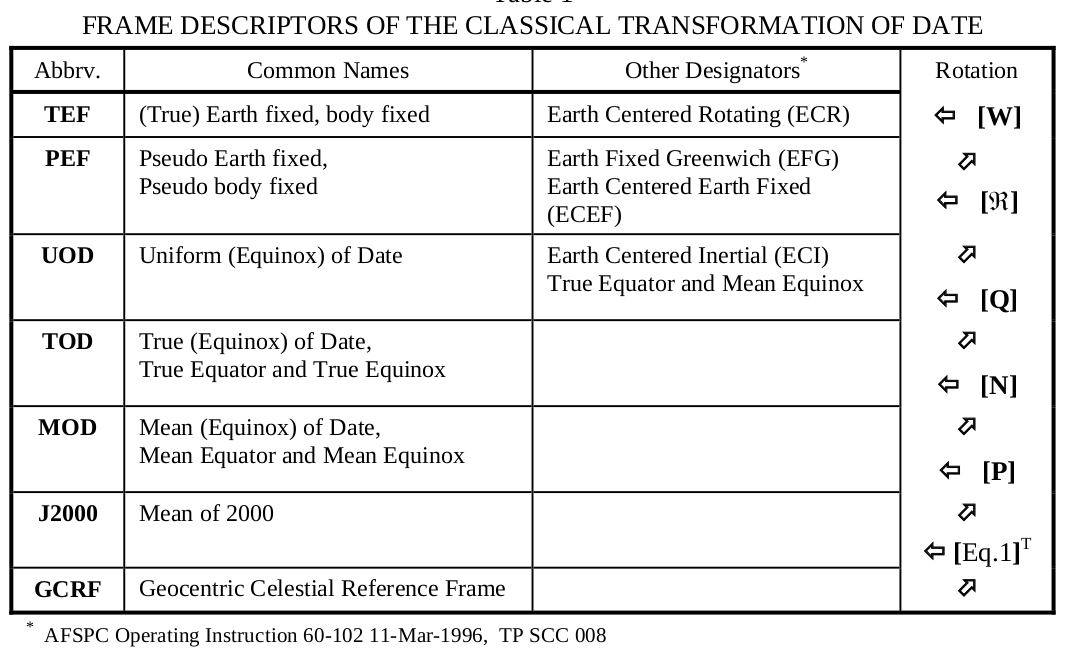
\includegraphics[width=0.7\textwidth]{imagenes/sistReferencias}
\end{figure}

En nuestro caso en particular, los datos que provee CODS se publican en el sistema TOD: True of Date (Verdadero de la \'epoca), mientras que los vectores de estado que genera el propagador SGP4 est\'an calculados en el sistema TEME: True Equator Mean Equinox (Ecuador Verdadero y Equinoccio Medio), tambi\'en denominado UOD (Uniform Equinox of Date).

Para la transformaci\'on de los datos de salida del SGP4 en el sistema TEME, al sistema TOD utilizamos la ecuaci\'on de los equinoccios, $EQ_{equinox}$, que nos permite transformar el equinoccio medio en el equinoccio verdadero.\\
Dado el vector de estado en el sistema TEME, $r_{_{TEME}}$, lo multiplicamos por la matriz de transformaci\'on en el eje z $Rot_{3}(EQ_{equinox})$ y obtenemos el vector de estado en el sistema TOD, $r_{_{TOD}}$.

\begin{equation}
 r_{_{TOD}} = [Q] r_{_{TEME}}
\end{equation}


 \[ Q =
\left( \begin{array}{ccc}
 cos(-EQ_{eqe}) & sin(-EQ_{eqe}) &  0 \\ 
 -sin(-EQ_{eqe}) & cos(-EQ_{eqe}) &  0 \\
 0 & 0 & 1
\end{array} \right) \] 


La ecuaci\'on de los equinoccios utiliza el modelo de nutaci\'on IAU-80 que considera los par\'ametros de nutaci\'on y los 106 coeficientes de Delaunay para el c\'alculo de la longitud $\Delta \Psi$ y la oblicuidad $\Delta \epsilon$.

\begin{equation}
 EQ_{eqe}=\Delta \Psi cos({\epsilon}) + 0.00264 \textquotedbl sin(\Omega_{(}) + 0.000063 \textquotedbl sin (2 \Omega_{(})
\end{equation}

Donde:

\begin{align*}
 \epsilon &= {\bar{\epsilon}} + \Delta \epsilon\\
 \Delta \Psi &= (A_{p} + A_{pl} tt) sin(a_{p_{i}})\\
 \Delta \epsilon &= (A_{e} + A_{el} tt) cos(a_{p_{i}})
\end{align*}

\begin{align*}
 tt &= (jd - 51544.5)/36525.0\\
 {\bar{\epsilon}} &= 84381.448 \textquotedbl - 46.8150 \textquotedbl tt - 0.00059 \textquotedbl tt^{2} + 0.001813 tt^{3}\\
 a_{p_{i}} &= a_{n1}M_{(}+a_{n2}M_{o}+a_{n3}\mu_{(}+a_{n4}D_{o}+a_{n5}\Omega_{(}
\end{align*}

Los coeficientes: $A_{p}$,$A_{pl}$,$A_{e}$,$A_{el}$,$A_{n_{i}}$ se extraen de la tabla de coeficientes de nutaci\'on de Seidelman(citar).

Y el resto de los par\'ametros se calcula seg\'un las expresiones:\\

\begin{align*}
 M_{(} & = M(tt)\\
 M_{o} & = M(tt)\\
 \mu_{(} &= \mu(tt)\\
 D_{o} &= D(tt)\\
 \Omega_{(} &= \Omega(tt)
\end{align*}

\section{Diferencias}
A partir de los datos de Misión. 

\begin{figure}[!h]
  \centering
  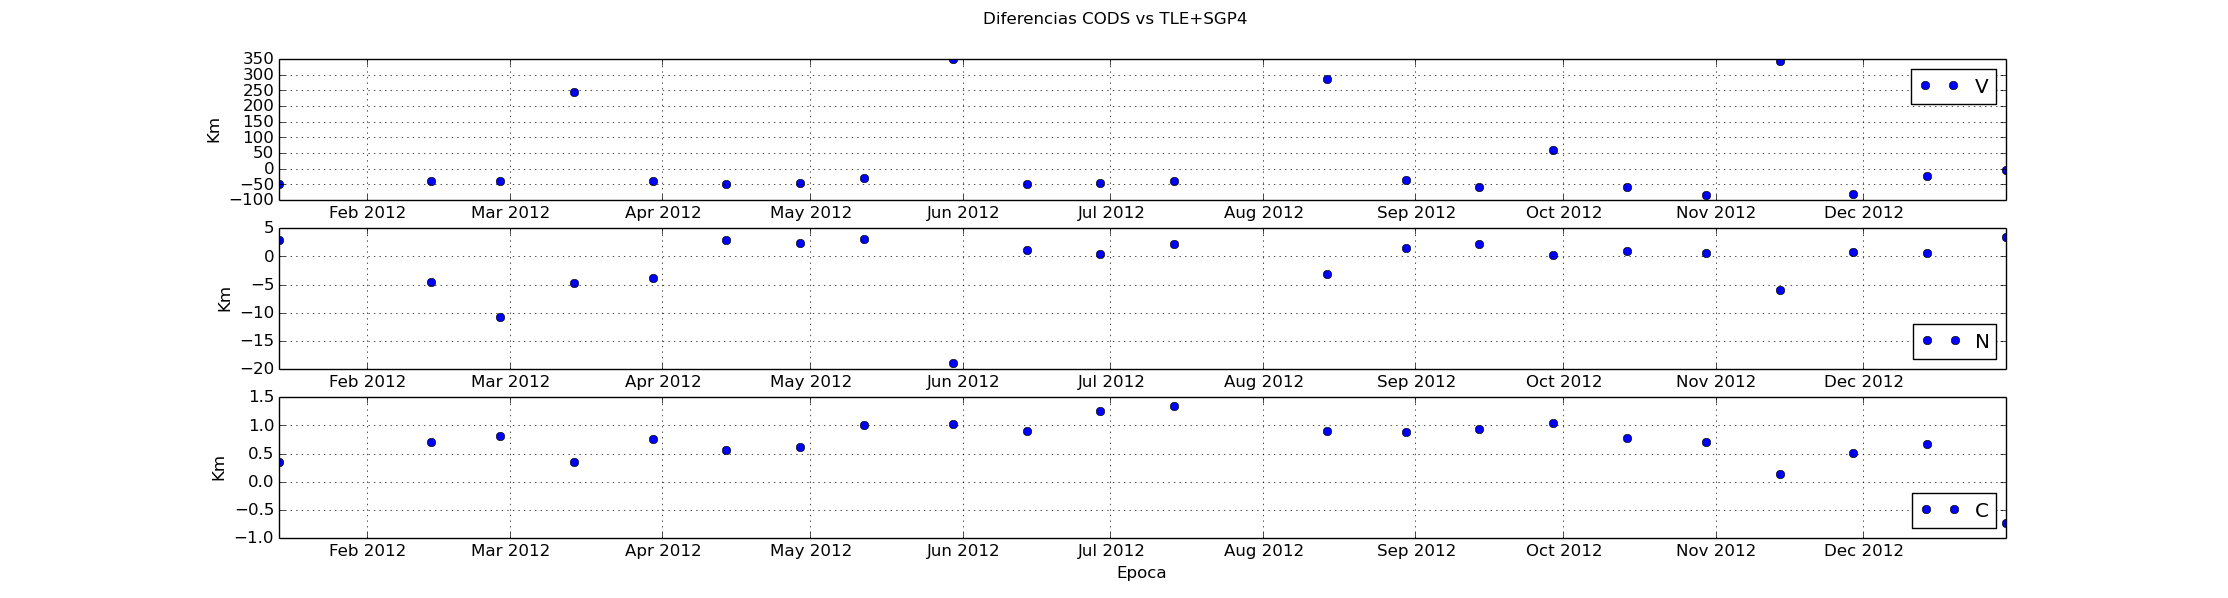
\includegraphics[width=\textwidth]{imagenes/sesgoTLE}
\end{figure}

\begin{itemize}
 \item Revisar escritura sobre datos CODS.
 \item Comparar defasaje inicial con defasaje de TLE respecto de GPS. (ver tendencias - empezar a diagramar los apédices)
 \item Comparar errores lineal vs cuadr\'atico.
\end{itemize}
